\documentclass[11pt,aspectratio=169]{beamer}

\usepackage{amsmath,amssymb,bm}
\usepackage{graphicx}
\usepackage{booktabs}

\usetheme{default}
\setbeamertemplate{navigation symbols}{}
\setbeamertemplate{headline}{}
\setbeamertemplate{footline}{}
\setbeamertemplate{frametitle}{%
  \vspace{0.25cm}%
  \insertframetitle\par
  \vspace{0.08cm}%
  \hrule
}
\setbeamercolor{normal text}{fg=black,bg=white}
\setbeamercolor{frametitle}{fg=black,bg=white}
\setbeamercolor{structure}{fg=black}
\setbeamersize{text margin left=0.7cm,text margin right=0.7cm}

\newcommand{\dd}{\,\mathrm{d}}
\newcommand{\Om}{\Omega}
\newcommand{\Gam}{\Gamma}
\newcommand{\norm}[1]{\left\lVert#1\right\rVert}
\newcommand{\bK}{\bm K}
\newcommand{\bF}{\bm F}
\newcommand{\bU}{\bm U}
\newcommand{\bx}{\bm x}
\newcommand{\bxi}{\bm\xi}
\newcommand{\bn}{\bm n}

\graphicspath{{figures/}}

\begin{document}

\begin{frame}[plain]
  \centering
  \vfill
  {\LARGE\bfseries Finite Elements in Two Dimensions\par}
  \vspace{0.45cm}
  {\large Linear triangular elements, basis-function support, and a diffusion computation\par}
  \vfill
\end{frame}

\section{Two-dimensional linear finite elements}

\begin{frame}{Lecture outline}
Today we will connect four parts of the two-dimensional finite element method:

\begin{enumerate}
  \item linear triangular elements and reference-to-physical mappings,
  \item a diffusion problem with Dirichlet and Neumann boundary conditions,
  \item global nodal basis functions and their support, and
  \item a FEniCSx solution and an $L^2$ error study under mesh refinement.
\end{enumerate}

\vspace{0.35cm}
We will state how local quantities enter $\bK$ and $\bF$, but we will not
repeat the assembly derivation from Chapter 5. The complete multidimensional
assembly procedure is in Chapter 6.
\end{frame}

\begin{frame}{From intervals to triangular meshes}
  \centering
  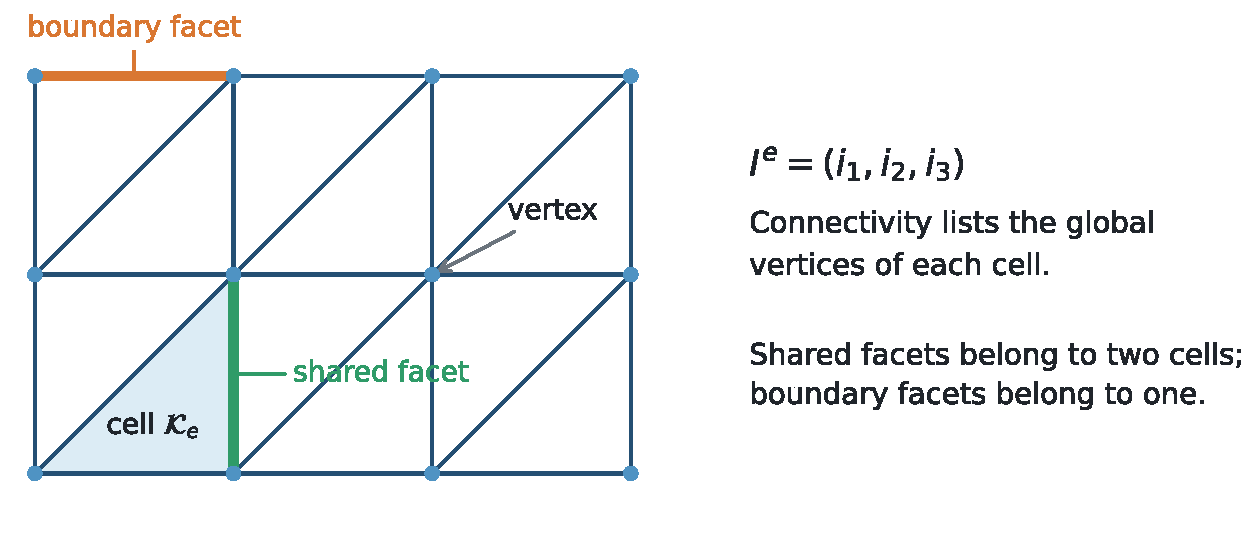
\includegraphics[width=0.88\textwidth]{c6_triangular_mesh_concepts.pdf}

  \vspace{0.08cm}
  A triangular mesh partitions $\Om$ into cells $\mathcal K_e$. Neighboring
  cells share vertices and edges, while boundary edges carry prescribed
  boundary data.
\end{frame}

\begin{frame}{The reference $P_1$ triangle}
\begin{columns}[T,onlytextwidth]
  \begin{column}{0.52\textwidth}
    \centering
    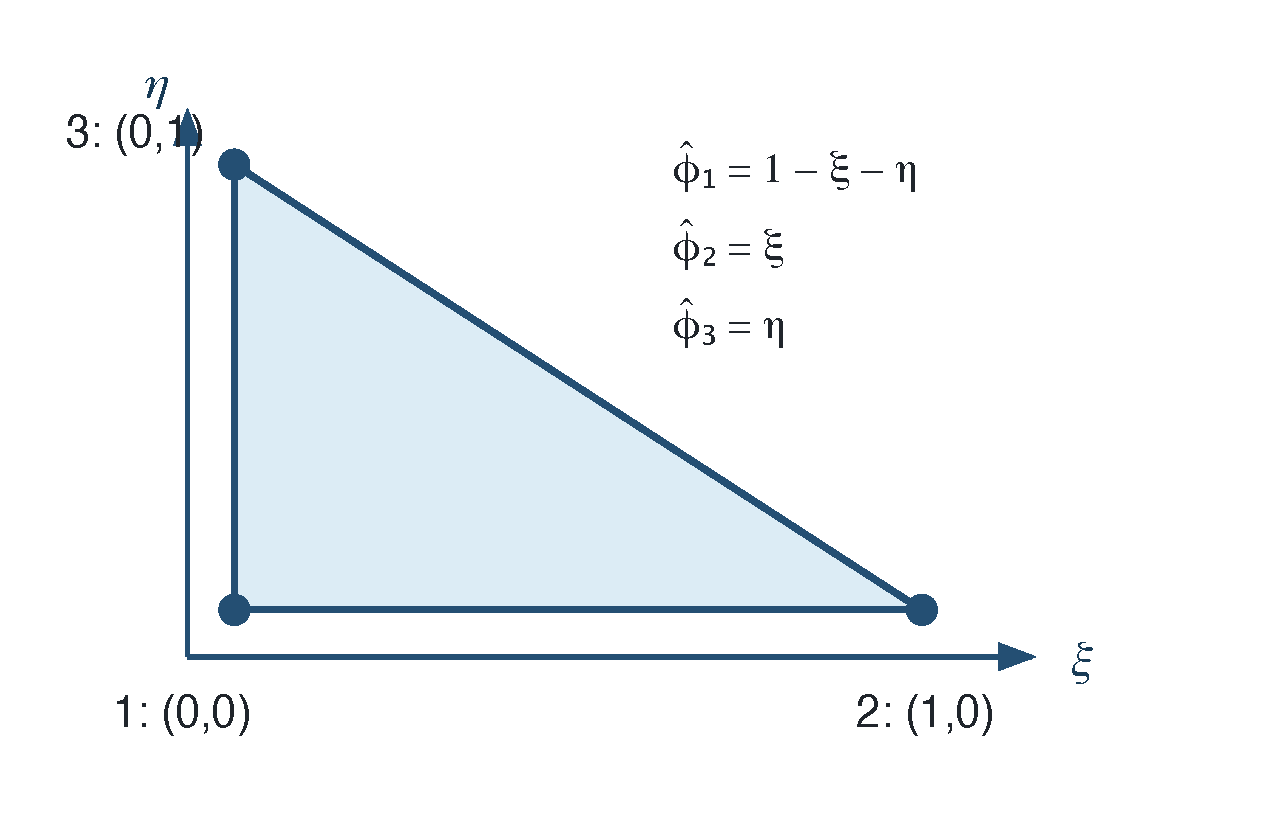
\includegraphics[width=\textwidth]{c6_reference_p1_triangle.pdf}
  \end{column}
  \begin{column}{0.45\textwidth}
    \[
      \widehat{\mathcal K}
      =\{(\xi,\eta):\xi\ge0,\ \eta\ge0,\ \xi+\eta\le1\}.
    \]
    The nodal basis functions satisfy
    \[
      \widehat\phi_a(\widehat\bx_b)=\delta_{ab},
      \qquad
      \sum_{a=1}^{3}\widehat\phi_a=1.
    \]
    Their gradients are constant on $\widehat{\mathcal K}$. Consequently, a
    $P_1$ triangle reproduces every affine scalar field exactly.
  \end{column}
\end{columns}
\end{frame}

\begin{frame}{Isoparametric reference-to-physical mapping}
  The geometry and finite element field use the same $P_1$ basis functions.
  This gives an \textbf{isoparametric mapping}.

  \centering
  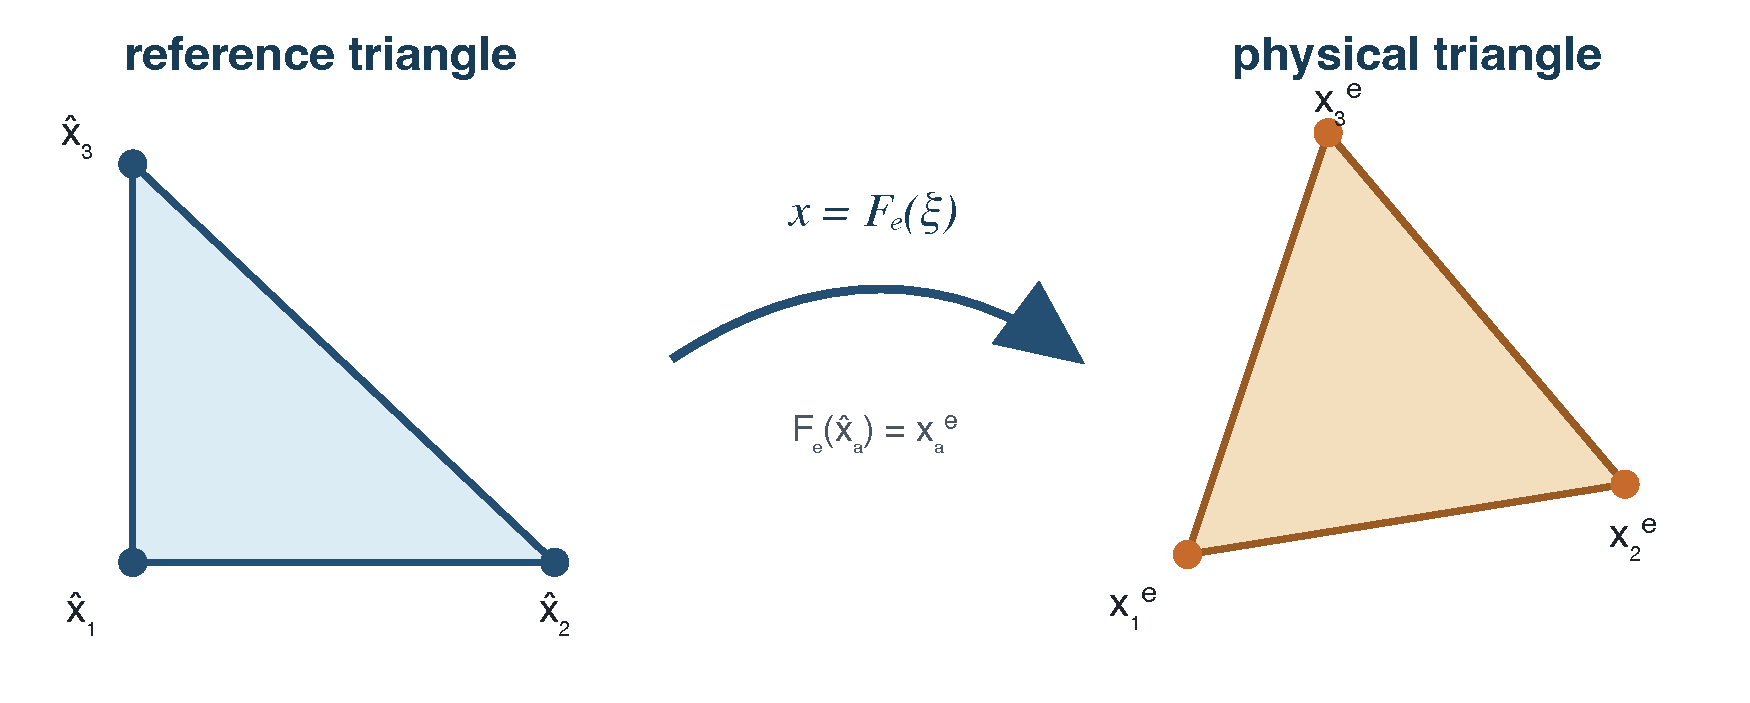
\includegraphics[width=0.62\textwidth]{c6_reference_triangle_mapping.pdf}

  \[
    \bx=F_e(\bxi)
    =\sum_{a=1}^{3}\widehat\phi_a(\bxi)\bx_a^e,
    \qquad
    \bm J_e=\frac{\partial\bx}{\partial\bxi}.
  \]
  \[
    \nabla_{\bx}\phi_a^e
    =\bm J_e^{-T}\nabla_{\bxi}\widehat\phi_a.
  \]
\end{frame}

\section{Diffusion problem and discrete equations}

\begin{frame}{Diffusion problem on the unit square}
\begin{columns}[T,onlytextwidth]
  \begin{column}{0.48\textwidth}
    \centering
    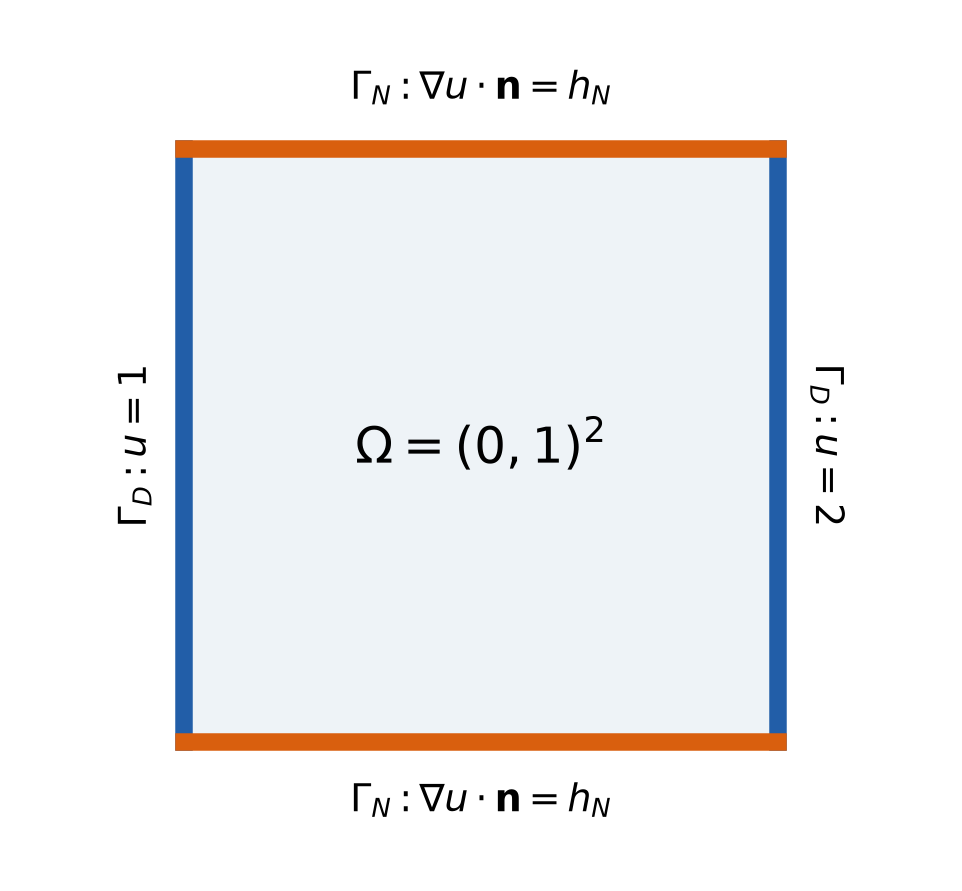
\includegraphics[width=0.96\textwidth]{c6_diffusion_domain_bc.png}
  \end{column}
  \begin{column}{0.49\textwidth}
    Let $\Om=(0,1)^2$. We solve
    \[
      -\Delta u=f\quad\text{in }\Om.
    \]
    The vertical sides form
    \[
      \begin{gathered}
        \Gam_D=\{x=0\}\cup\{x=1\},\\
        u=g\quad\text{on }\Gam_D.
      \end{gathered}
    \]
    The horizontal sides form
    \[
      \begin{gathered}
        \Gam_N=\{y=0\}\cup\{y=1\},\\
        \nabla u\cdot\bn=h_N\quad\text{on }\Gam_N.
      \end{gathered}
    \]
  \end{column}
\end{columns}
\end{frame}

\begin{frame}{Exact solution and problem data}
Choose
\[
  u_\star(x,y)=1+x+x(1-x)\sin(\pi y).
\]
Substitution into the differential equation and boundary conditions gives
\[
  \begin{aligned}
    f(x,y)&=\bigl[2+\pi^2x(1-x)\bigr]\sin(\pi y),\\
    g(x,y)&=1+x && \text{on }\Gam_D,\\
    h_N(x,y)&=-\pi x(1-x) && \text{on }\Gam_N.
  \end{aligned}
\]
Thus $u=1$ on the left edge and $u=2$ on the right edge. The prescribed
normal flux is nonzero on the interiors of the top and bottom edges.
\end{frame}

\begin{frame}{Variational and finite element problems}
Define
\[
  \mathcal U_g
  =\{w\in H^1(\Om):w=g\text{ on }\Gam_D\},
  \qquad
  \mathcal V_0
  =\{v\in H^1(\Om):v=0\text{ on }\Gam_D\}.
\]
The variational problem is
\[
  \text{find }u\in\mathcal U_g:\qquad
  \int_\Om\nabla u\cdot\nabla v\,\dd\bx
  =
  \int_\Om f v\,\dd\bx
  +\int_{\Gam_N}h_Nv\,\dd s
  \quad\forall v\in\mathcal V_0.
\]

The finite element problem restricts the trial and test functions to the
continuous piecewise-linear space $\mathcal V_h$:
\[
  u_h\in\mathcal U_{h,g_h},
  \qquad
  v_h\in\mathcal V_{h,0}.
\]
\end{frame}

\begin{frame}{The global algebraic system}
Write the finite element field as
\[
  u_h=\sum_{j=1}^{N_n}U_j\phi_j.
\]
Testing with the free nodal basis functions gives
\[
  \bK\bU=\bF,
\]
with entries
\[
  K_{ij}=\int_\Om\nabla\phi_j\cdot\nabla\phi_i\,\dd\bx,
  \qquad
  F_i=\int_\Om f\phi_i\,\dd\bx
      +\int_{\Gam_N}h_N\phi_i\,\dd s.
\]

In practice, the code computes cell matrices $\bK^e$, cell load vectors
$\bF^e$, and boundary-edge contributions. Connectivity identifies the rows and
columns of $\bK$ and $\bF$ that receive these local entries. Chapter 6 gives
the complete assembly construction.
\end{frame}

\section{Global basis functions and support}

\begin{frame}{A global nodal basis function}
Let $\bx_i$ be mesh node $i$. The global basis function $\phi_i$ satisfies
\[
  \phi_i(\bx_j)=\delta_{ij}.
\]
It equals one at node $i$, equals zero at every other mesh node, and is linear
on each triangle.

The incident-cell set is
\[
  \mathcal E(i)
  =\{e:\bx_i\text{ is a vertex of }\mathcal K_e\}.
\]
Then
\[
  \operatorname{supp}(\phi_i)
  =\bigcup_{e\in\mathcal E(i)}\overline{\mathcal K_e}.
\]

On every triangle outside this patch, all three nodal values of $\phi_i$ are
zero, so the linear function is zero throughout that triangle.
\end{frame}

\begin{frame}{Basis-function support on an 18-triangle mesh}
  \centering
  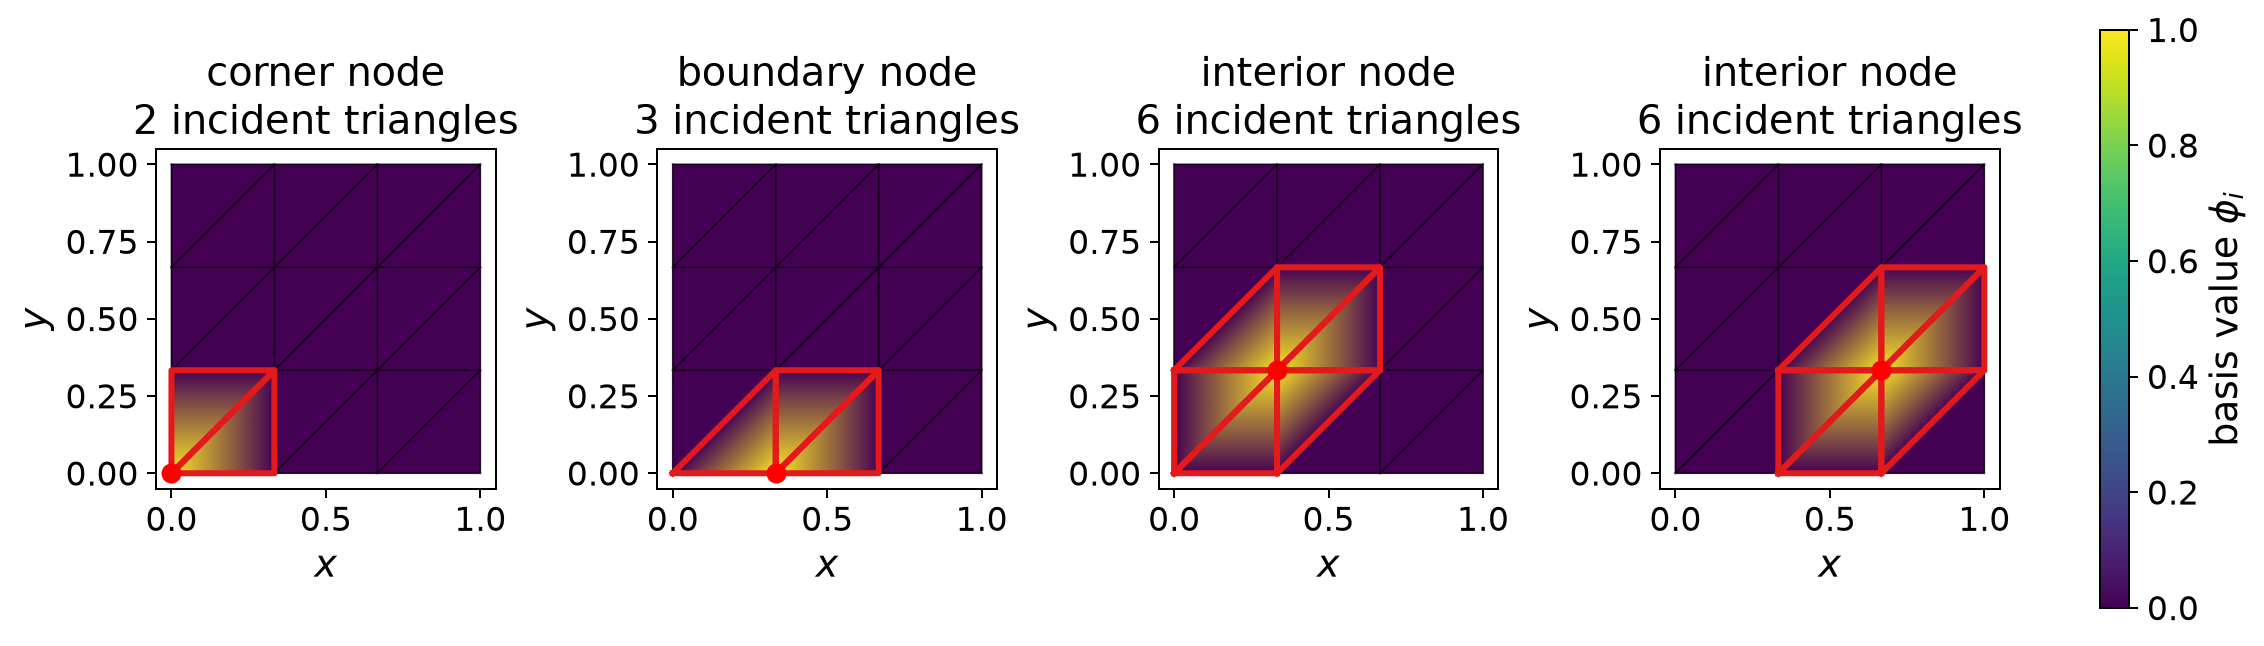
\includegraphics[width=0.98\textwidth]{c6_basis_support.png}

  \vspace{-0.08cm}
  Each plot sets one nodal coefficient equal to one and all others equal to
  zero. The highlighted patch consists exactly of the elements incident on the
  selected node.
\end{frame}

\begin{frame}{Support and the stiffness matrix}
The stiffness entry
\[
  K_{ij}=\int_\Om\nabla\phi_j\cdot\nabla\phi_i\,\dd\bx
\]
can be nonzero only where the supports of $\phi_i$ and $\phi_j$ overlap.
Therefore,
\[
  \operatorname{supp}(\phi_i)\cap
  \operatorname{supp}(\phi_j)=\varnothing
  \quad\Longrightarrow\quad
  K_{ij}=0.
\]

For linear triangles, two nodal basis functions overlap only when their nodes
belong to at least one common triangle. This local interaction produces a
sparse global matrix even when the mesh contains many degrees of freedom.
\end{frame}

\begin{frame}{Sparsity of the stiffness matrix}
\begin{columns}[T,onlytextwidth]
  \begin{column}{0.56\textwidth}
    \centering
    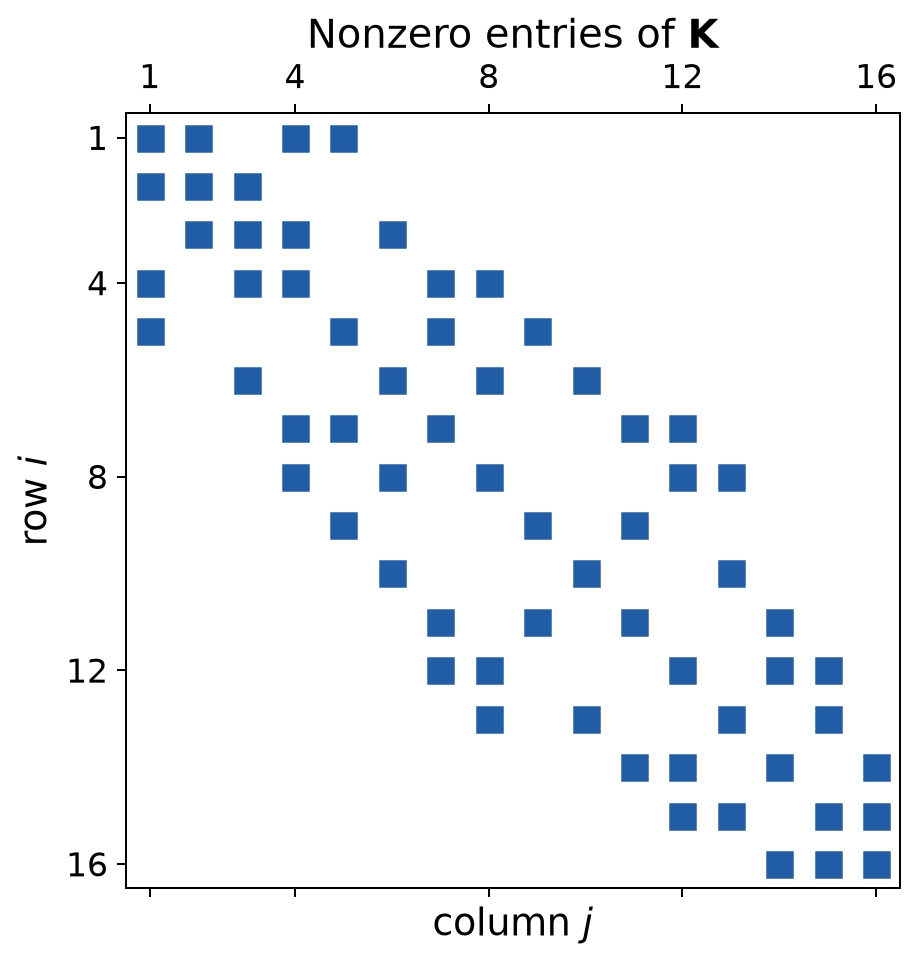
\includegraphics[height=0.68\textheight,keepaspectratio]{c6_stiffness_sparsity.png}
  \end{column}
  \begin{column}{0.41\textwidth}
    The 18-triangle mesh has 16 nodal degrees of freedom, so $\bK$ is a
    $16\times16$ matrix.

    \vspace{0.25cm}
    A dot marks a nonzero entry $K_{ij}$. Nonzero off-diagonal entries occur
    only when nodes $i$ and $j$ belong to a common triangle.

    \vspace{0.25cm}
    Each node interacts with only a small part of the mesh. The resulting
    stiffness matrix is symmetric and sparse.
  \end{column}
\end{columns}
\end{frame}

\section{FEniCSx computation and refinement}

\begin{frame}{FEniCSx demonstration sequence}
The live notebook follows the same mathematical order:

\begin{enumerate}
  \item Create the triangular mesh and the continuous $P_1$ space.
  \item Locate $\Gam_D$ and $\Gam_N$ and assign the boundary data.
  \item Define the trial function, test function, and variational forms.
  \item Solve the linear system for the nodal coefficients.
  \item Compare $u_h$ with $u_\star$ using the $L^2(\Om)$ error.
\end{enumerate}

\vspace{0.25cm}
We first use a separate $3\times3$ subdivision to inspect basis functions.
The convergence study begins with four triangles and then halves the mesh size
twice.
\end{frame}

\begin{frame}{Solution on four triangles}
\begin{columns}[T,onlytextwidth]
  \begin{column}{0.56\textwidth}
    \centering
    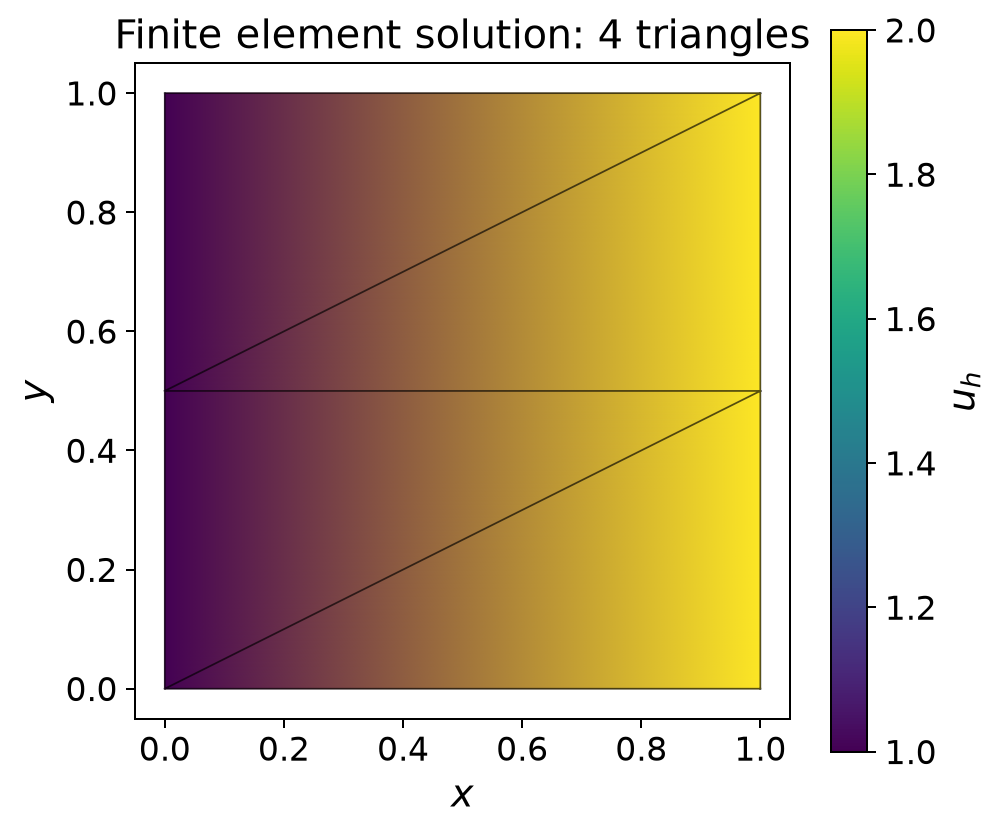
\includegraphics[width=0.92\textwidth]{c6_diffusion_4_triangles.png}
  \end{column}
  \begin{column}{0.41\textwidth}
    The mesh has six nodal degrees of freedom.

    \vspace{0.2cm}
    Every node lies on $x=0$ or $x=1$, where the prescribed values are
    $1$ and $2$. The coarse finite element field cannot yet represent the
    interior $x(1-x)\sin(\pi y)$ variation.

    \vspace{0.2cm}
    Measured error:
    \[
      \norm{u_\star-u_h}_{L^2(\Om)}
      =1.291\times10^{-1}.
    \]
  \end{column}
\end{columns}
\end{frame}

\begin{frame}{Uniform mesh refinement}
  \centering
  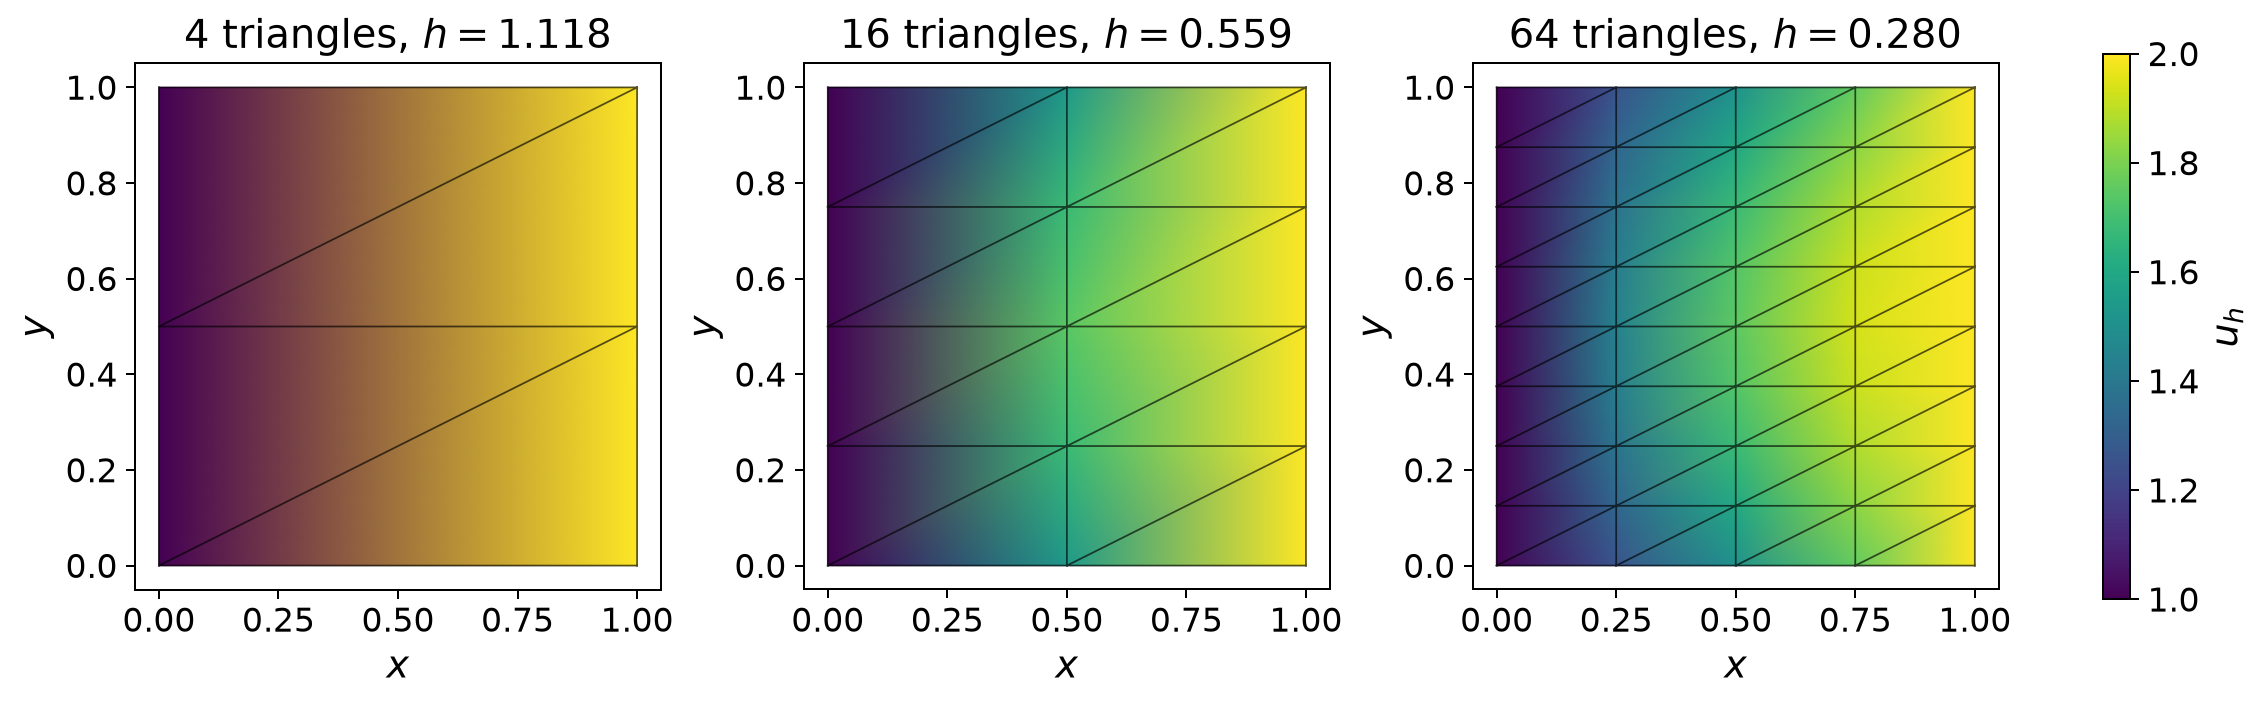
\includegraphics[width=0.98\textwidth]{c6_diffusion_refinement.png}

  \vspace{-0.08cm}
  The three meshes contain 4, 16, and 64 triangles. Doubling the subdivisions
  in each coordinate changes the mesh size from $h$ to $h/2$ and then to
  $h/4$.
\end{frame}

\begin{frame}{$L^2$ error under refinement}
\begin{columns}[T,onlytextwidth]
  \begin{column}{0.57\textwidth}
    \centering
    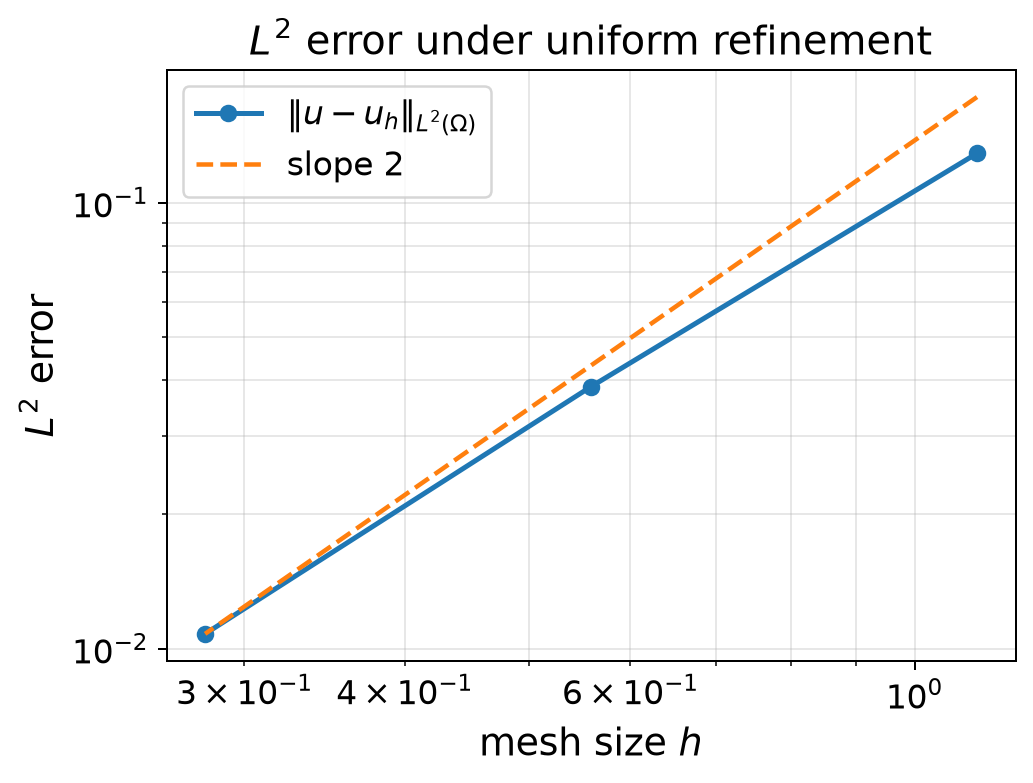
\includegraphics[width=0.96\textwidth]{c6_diffusion_l2_convergence.png}
  \end{column}
  \begin{column}{0.40\textwidth}
    \centering
    \begin{tabular}{ccc}
      \toprule
      triangles & $h$ & $L^2$ error\\
      \midrule
      4  & 1.118 & $1.291\times10^{-1}$\\
      16 & 0.559 & $3.870\times10^{-2}$\\
      64 & 0.280 & $1.079\times10^{-2}$\\
      \bottomrule
    \end{tabular}

    \vspace{0.35cm}
    The observed rates are $1.74$ and $1.84$. The meshes are still coarse, but
    the error approaches the second-order $L^2$ behavior expected for smooth
    solutions and linear elements.
  \end{column}
\end{columns}
\end{frame}

\begin{frame}{What to retain from today}
\begin{itemize}
  \item A two-dimensional $P_1$ function is linear on each triangle and
  continuous across shared edges.
  \item Reference basis functions and the element map provide basis values,
  physical gradients, and element integration.
  \item Each global nodal basis function is supported only on the triangles
  incident on its node.
  \item The discrete problem has the form $\bK\bU=\bF$; local matrices and
  vectors enter the global system through connectivity.
  \item Uniform refinement reduces the measured $L^2$ error for the diffusion
  problem.
\end{itemize}

\vspace{0.2cm}
Read Chapter 6 for the complete assembly procedure, quadrature rules,
quadrilateral and three-dimensional elements, and vector-valued elasticity.
\end{frame}

\end{document}
